\documentclass[conference]{IEEEtran}

\usepackage{pdfpages}
\usepackage{url}

% correct bad hyphenation here
\hyphenation{op-tical net-works semi-conduc-tor}

\begin{document}
\title{Report for Wood's paper: 
The Feasibility of Magnetic Recording at 10 Terabits Per Square Inch on Conventional Media}

\author{\IEEEauthorblockN{Kamoliddin Mavlonov}
\IEEEauthorblockA{Graduate School of Science and Engineering\\
Ehime University\\
3 Bunkyou-cho Matsuyama Ehime 790-8577, Japan\\
kamol@koblab.cs.ehime-u.ac.jp}}

\maketitle

\begin{abstract}
This report is purely based on my own comprehension of this paper.
\end{abstract}

\IEEEpeerreviewmaketitle

% Introduction
\section{Introduction}
In 2000, Wood publishes a paper: The Feasibility of Magnetic Recording at 1 Terabits Per Square Inch~\cite{Wood2000}. It says, that conventional recording would reach a limit at around 1 Terabit/in$^2$.

However, in 2009, he admits~\cite{Wood2009} the current hard disk drive (HDD) technology is already reaching this limit. Wood is right that to assure continued capacity growth in HDD need alternative technologies: heat-assisted magnetic recording (HAMR)~\cite{Rottmeyer} and bit patterned media (BPM)~\cite{Terris}. 

Toward proof of the concept, the Advanced Storage Technology Consortium (ASTC)~\cite{ASTC} released the 2014 roadmap for HDD area density as shown in Fig.\,\ref{fig_astc}.

As you can see from Fig.~\,\ref{fig_astc}, current HDD technology is Perpendicular recording\

\begin{figure}[!hbt]
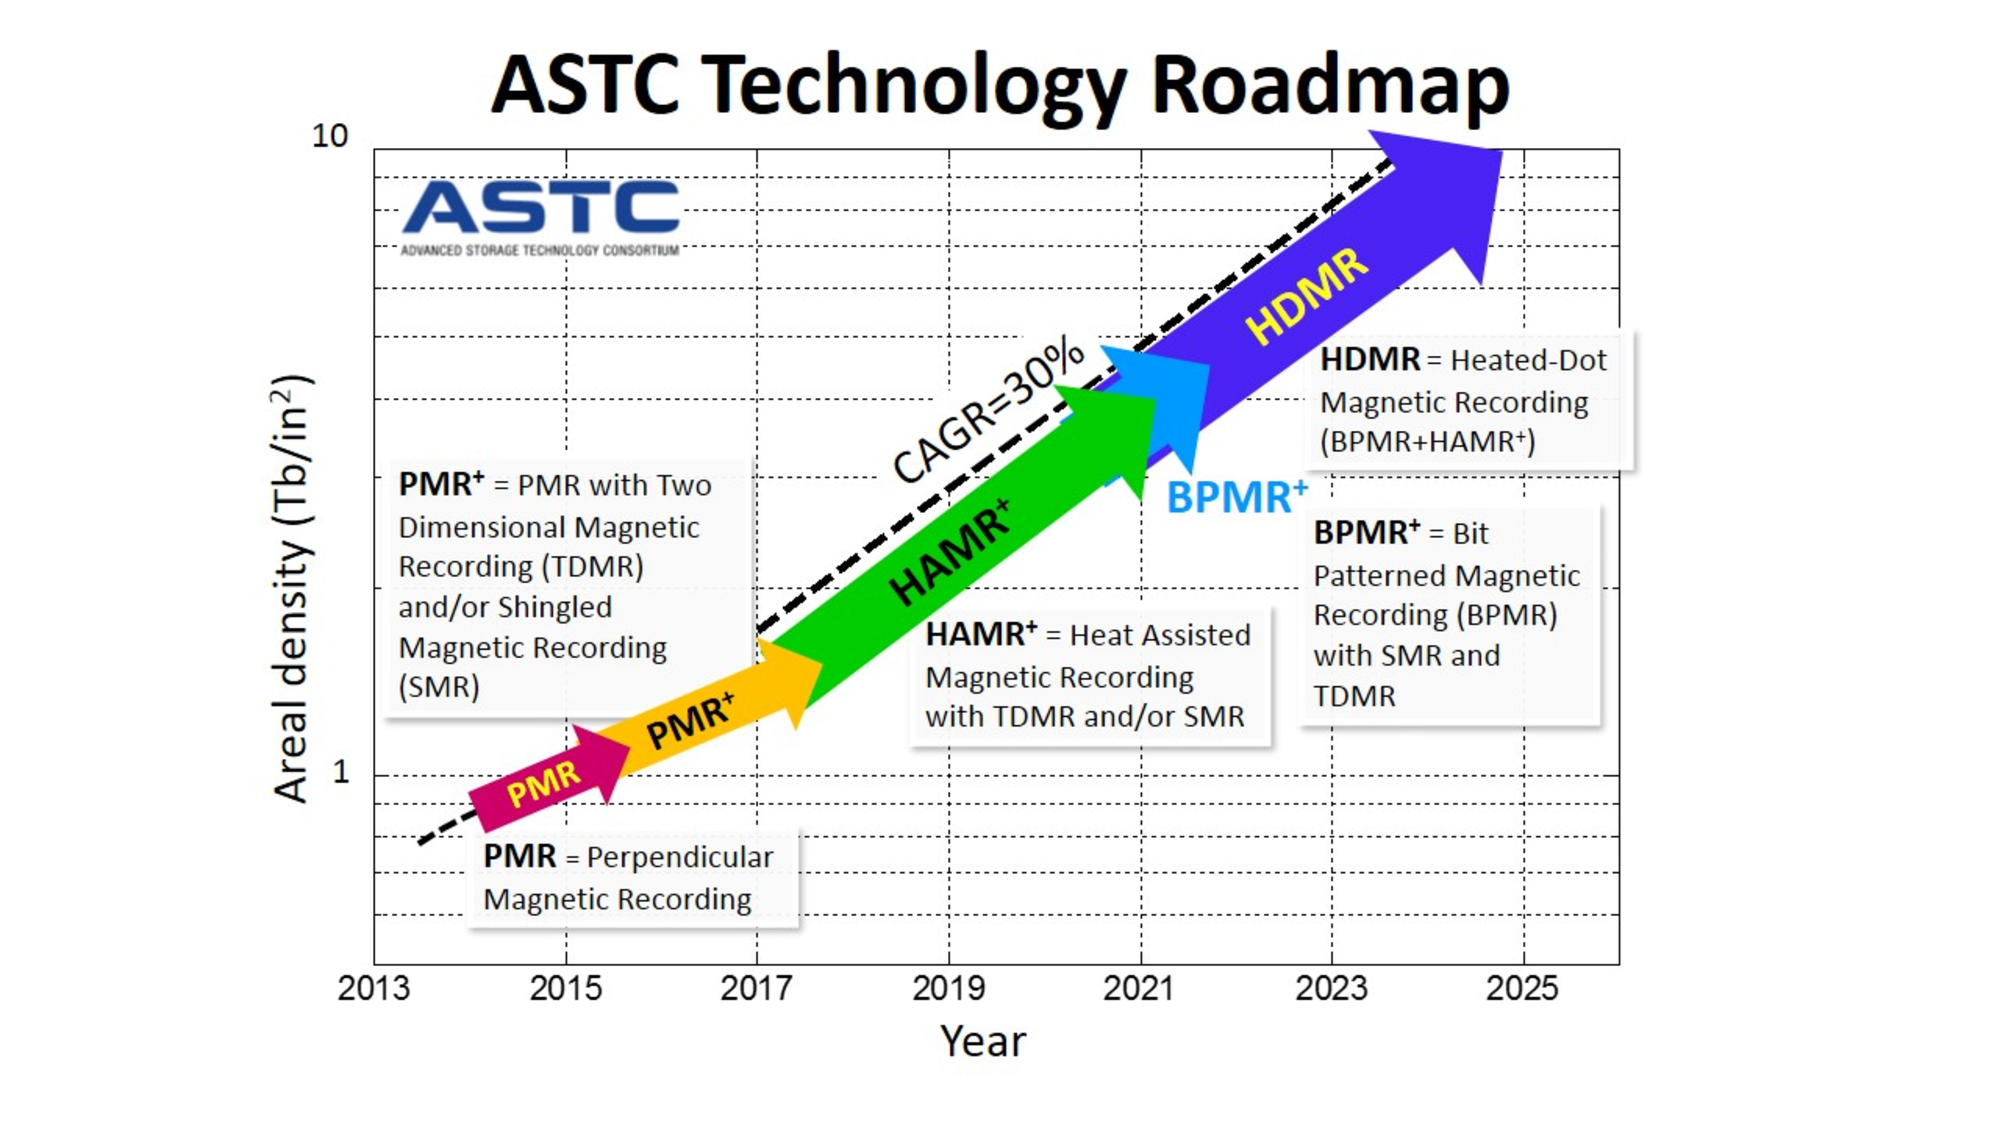
\includegraphics[height=0.25\textheight]{ASTC}
\caption{Data synchronization between two devices}
\label{fig_astc}
\end{figure}

\section{Shingled Writing}

\section{Two-Dimensional read-back}
TDMR architecture also helps to achieve the increased aerial density of 10Tb/in$^2$. It is the combination of Shingled writing and the two dimensional readback.~\cite{IEEE_HITACHI} Since the Shingled writing writes by overlapping the previously written track, it is quite challenging to read back. The conventional read for the shingled writing is more erroneous because of Inter-track Interference (ITI). So for SMR Writing, 2D readback is used to minimise the ITI. TDMR uses the whole of 2D array bits in different track as a single unit. This can be achieved by the following ways.
\begin{itemize}
	\item Allowing multiple passes using single read head.
	\item Using array of read heads.
\end{itemize}

Using single read head for each pass the readback is stored in the memory. After storing all the readback for each pass then processing of the data can be done. So it would increase memory and also would considerably increase the latency. On the other hand by using multiple read heads parallel readbacks can be stored in the memory and can be processed with less latency than the single head.~\cite{Elidrissi}

The read/write channel model of TDMR has 3 components such as recording medium generation, data writing process and readback process. The following are the 3 models which is quite popular for the read channel models of the TDMR~\cite{Krishnan}\cite{Vasic}
\begin{itemize}
	\item Voronoi model
	\item Discrete Grain model
	\item Error erasure model
\end{itemize}



\subsection{Subsection Heading Here}
Subsection text here.


\subsubsection{Subsubsection Heading Here}
Subsubsection text here.



\section{Conclusion}
The conclusion goes here.


% use section* for acknowledgment
\section*{Acknowledgment}


The authors would like to thank...

% set second argument of \begin to the number of references
% (used to reserve space for the reference number labels box)
\begin{thebibliography}{1}

\bibitem{Wood2000}
R.~Wood, \emph{The feasibility of magnetic recording at 1 terabit per square
inch}, IEEE Trans. Magn., vol. 36, pp. 36–42, Jan. 2000.

\bibitem{Rottmeyer}
R.~Rottmeyer et al., \emph{Heat-assisted magnetic recording}, IEEE Trans.
Magn., vol. 42, no. 10, pp. 2417–2421, Oct. 2006.

\bibitem{Terris}
B.~Terris, T. Thomson, and G. Hu, \emph{Patterned media for future magnetic
data storage}, Microsyst. Technol., vol. 13, no. 2, pp. 189–196, Nov.
2006.

\bibitem{Wood2009}
R.~Wood, M. Williams, A. Kavcic, J. Miles, \emph{The Feasibility of Magnetic Recording at 10 Terabits Per Square Inch on Conventional Media}, IEEE Trans. Magn., vol. 45, pp. 917-923, Feb. 2009.

\bibitem{ASTC}
ASTC Technology Roadmap - 2014 v8, \url{http://idema.org/?page_id=416}, 2014.

\bibitem{HGST}
\emph{Perpendicular Magnetic Recording Technology}, HGST, a Western Digital company, Nov, 2007.


\end{thebibliography}


% that's all folks
\end{document}